\chapter{Implementation}
\label{chap:prog}
\begin{figure}[ht]
\centering
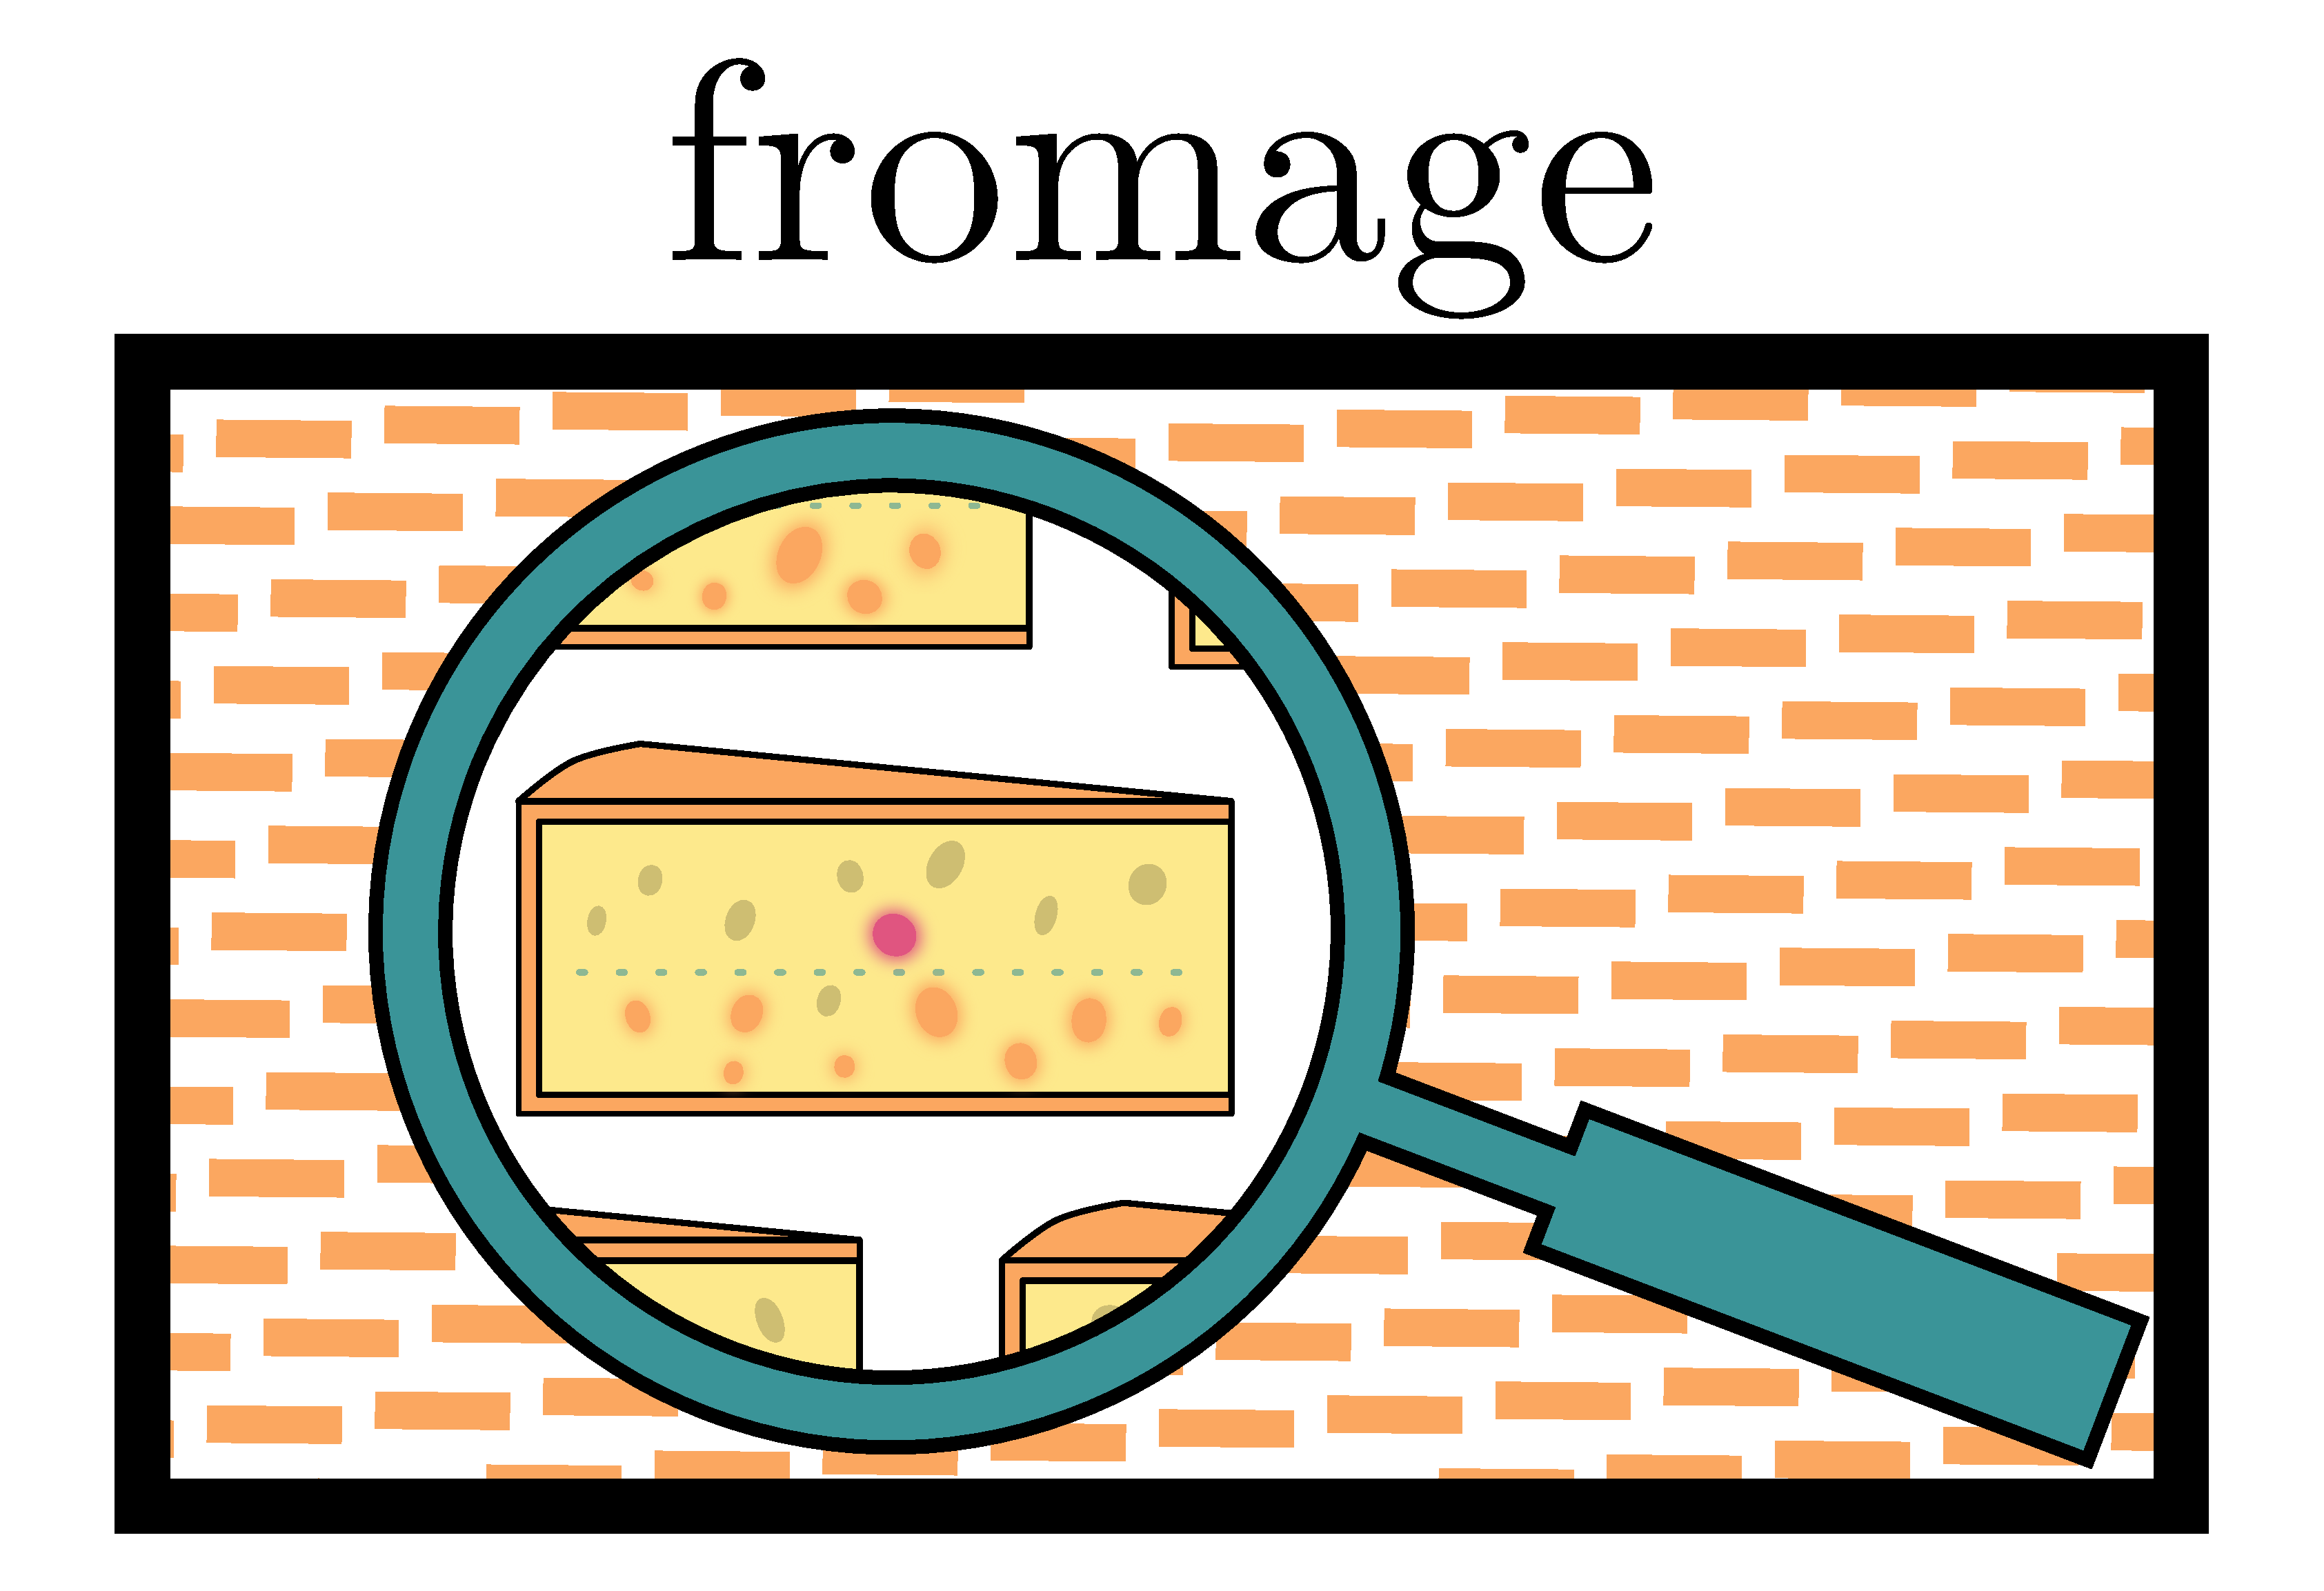
\includegraphics[width=7cm]{Chapters/6Implementation/toc.pdf}
\end{figure}



\section{Introduction}

Chapter \ref{chap:jctc} should provide enough evidence that studying the photochemistry of some molecular crystals at the finite scale is a sensible idea. In fact, the structural features which are relevant to these systems are of the scale of the aggregate, ranging from monomer conformation and dimer packing all the way to molecular cluster shape.

The methodology already existing to model finite size molecular aggregates can therefore in part be repurposed to model periodic molecular crystals when dealing with excited state processes. The commonplace approach to investigating molecular crystals\textemdash{}using periodic electronic structure codes\textemdash{}should thus be complemented by adequately extending molecular aggregate methods for the excited state.

The generation and analysis of these aggregate nuclear configurations is often separated from the codes which produce their corresponding electronic structure. Whilst the former tasks are typically less computationally demanding than the latter one and therefore might be added as an auxiliary feature to a larger code (e.g. Crystal17\cite{Dovesi2018}), they often require a degree of flexibility which situates them more comfortably in the realm of the programming library. Indeed the bridging of scales between the periodic crystal, finite cluster, dimer, and monomer is challenging to generalise due to the formidable conformational variety of organic molecules.

An optimal strategy is therefore to provide modular tools for the investigator to tailor to their system, accompanied by ready-made scripts which compile those tools for use in ubiquitous cases. In this way, non-expert users are able to use the program's principal features with a reliable degree of robustness, whilst more comfortable users can repurpose and extend the code to better suit fringe cases.

There exists a variety of computational chemistry scripting libraries for different tasks, with the ecosystem in rapid development. Their promise is to optimise and standardise the research workflow for increasingly specialised operations thanks to robust, tailored tools. The Cambridge Structural Database (CSD) Python API\cite{Groom2016} focuses on crystallographic property analysis, accessing its associated database. The Atomic Simulation Environment (ASE)\cite{Larsen2017} specialises in interfacing with numerous electronic structure codes and communicates with them \textit{via} Python scripting or a GUI. RDKit\cite{rdkit} provides programming tools for general purpose chemoinformatics and is itself used in numerous child libraries. Chemshell provides additive QM:MM interfaces between electronic structure and forcefield codes.\cite{Lu2019} Libra is a library designed for the development of quantum and classical dynamics.\cite{Akimov2016} To our knowledge, there still lacks a library dedicated to the examination of photochemistry in molecular aggregates and crystals, exploiting the overlap in methodology between the two materials.

To address this, we offer the FRamewOrk for Molecular AGgregate Excitations (\texttt{fromage}). \texttt{fromage} is a standalone Python library, accompanied by ready-to-use command line scripts destined to facilitate the study of molecular aggregates in the excited state. They are summarised in Figure \ref{fig:features}. The program is tested for Python 2.7 and 3.6, though the authors do not guarantee backwards compatibility with Python 2 in future releases. For geometry manipulation routines, the program only relies on the unit cell's Cartesian structure and lattice vectors. From this information, the user can obtain unique dimer configurations, molecular clusters and general structural information.

All of the electronic structure calculations are performed by popular quantum chemistry programs. Currently, interfaces are provided to run calculations in \texttt{DFTB+},\cite{Aradi2007} \texttt{Gaussian},\cite{g16} \texttt{Molcas},\cite{Aquilante2016} and \texttt{Turbomole}.\cite{TURBOMOLE} By delegating these calculations to different programs, their results can be combined into hybrid energy expressions. Thus \texttt{fromage} can perform ONIOM calculation\textemdash{}including those discussed in Chapter \ref{chap:jctc}\textemdash{}whilst taking advantage of the diversity of modelling methods of several programs instead of only one.\cite{Rivera2019}

\texttt{fromage} has been used to study various QM:QM' electrostatic embedding schemes for applications in photoactive molecular crystals,\cite{Rivera2019} the aggregation induced emission process in propeller-shaped molecules,\cite{Stojanovic2019} and the design principles for proton transfer luminescent materials.\cite{Dommett2019} 

Users interested in using the program should refer primarily to the full documentation, available at \href{https://fromage.readthedocs.io/}{https://fromage.readthedocs.io/}. It contains tutorials, and technical instructions for all primary operations. This chapter presents an overview of the program's capabilities, though readers wishing to use them should refer primarily to the documentation. First we describe the program structure, illustrated by basic usage examples. Then we enumerate its principal features, namely geometric analysis, exciton coupling evaluation and ONIOM QM:QM' models. This final point addresses the problems of inadequate implementation for cluster models in organic molecular crystal photochemistry discussed in Section \ref{sec:prob_imp}.

\begin{figure}[ht]
  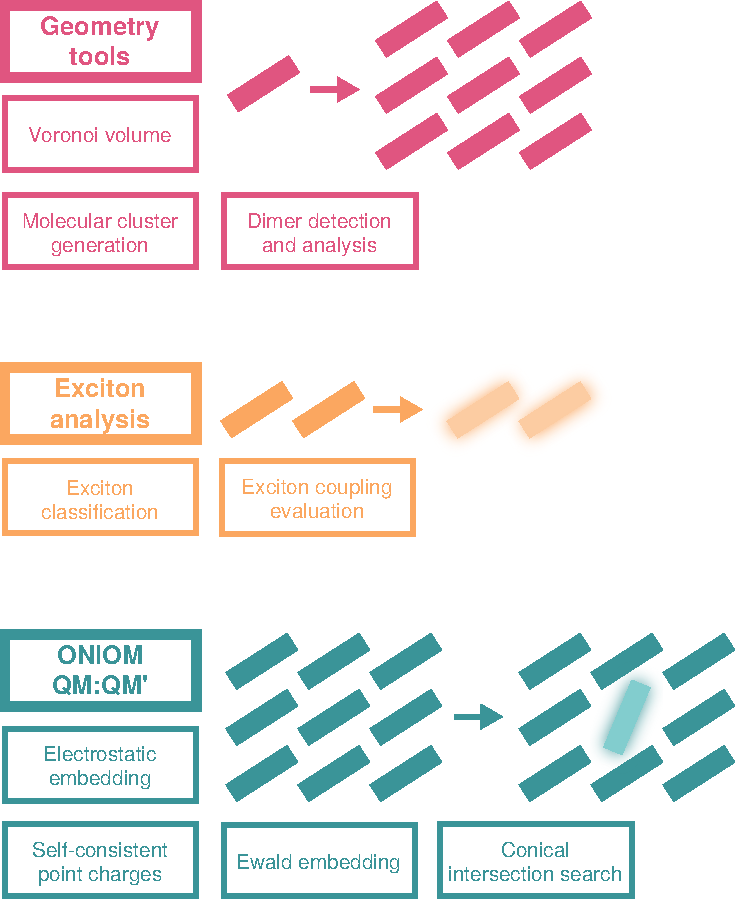
\includegraphics[width=9cm]{Chapters/6Implementation/scheme.pdf}
  \caption{Principal features of \texttt{fromage}.}
  \label{fig:features}
\end{figure}

\section{Program Structure}
\subsection{Principal Classes}
\texttt{fromage} makes use of two main classes in most of its operations, \texttt{Atom} and \texttt{Mol}. An \texttt{Atom} object is defined as a point in Cartesian space with associated physical properties. If the point is to represent an atom, supplying its element string provides standard properties such as covalent radius or atomic mass. The partial charge can also be specified, which can become useful in representing both atoms and point charges.

In practice, the user has little direct interaction with \texttt{Atom} objects. Instead they manipulate \texttt{Mol} objects, which contain a list of the former. \texttt{Mol} extends common Python list methods \textit{via} composition, allowing for intuitive appending, indexing, iterating etc. but also provides methods to manipulate molecular aggregate geometries and unit cells. \texttt{Mol} objects can be created explicitly or generated from a typical geometry file such as \texttt{.xyz}. For instance, one may generate a molecular cluster and a supercell from unit cell information as illustrated in Figure \ref{fig:script}.

\begin{figure}[ht]
\centering
  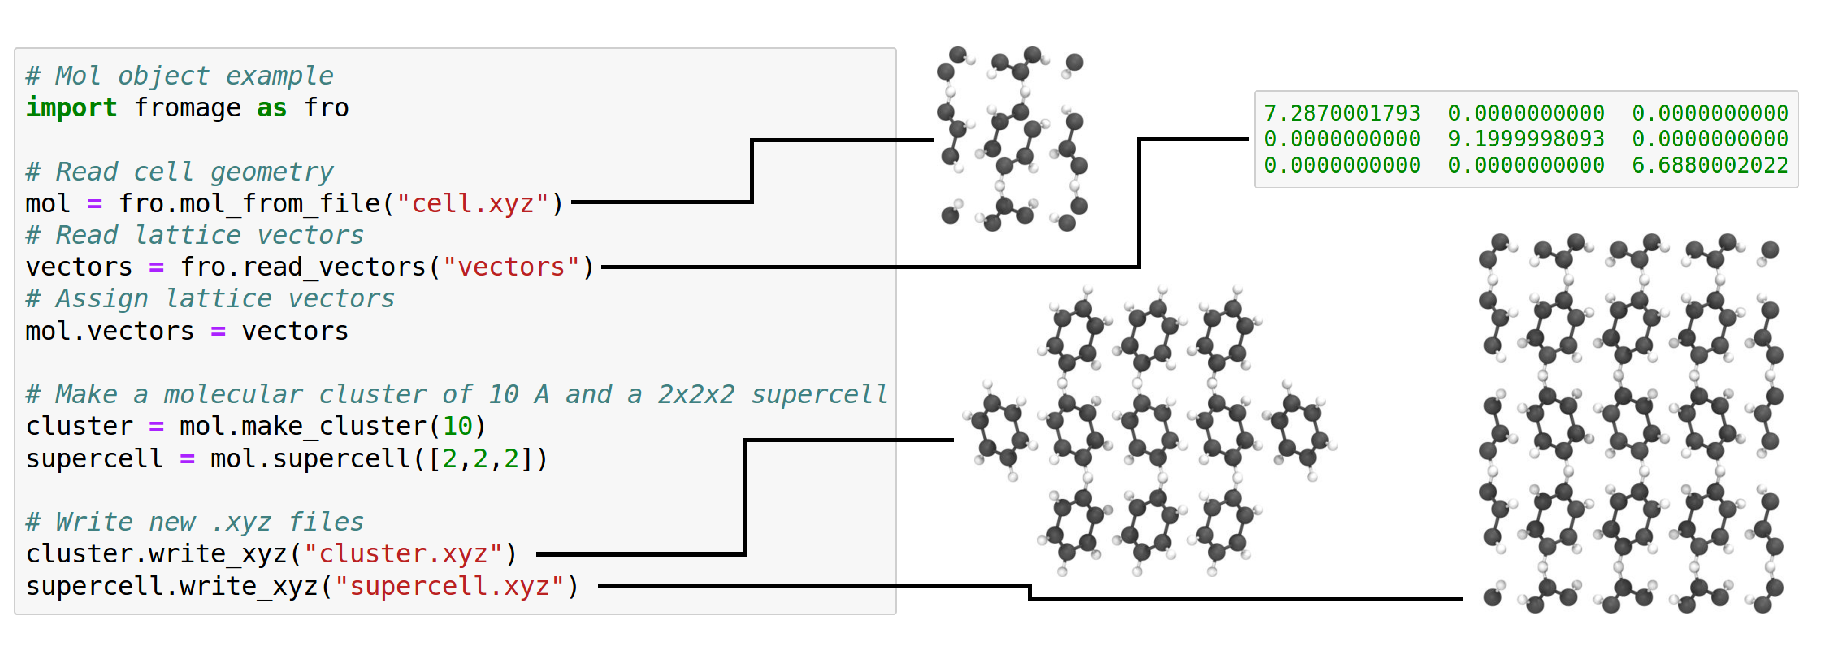
\includegraphics[width=\textwidth]{Chapters/6Implementation/script_fig.pdf}
  \caption{Example of use of \texttt{fromage} as a Python library. The three dimensional structures are shown in orthographic projection.}
  \label{fig:script}
\end{figure}


Apart from the constituent atoms and lattice vectors, \texttt{Mol} also has attributes pertaining to the definition of a bond within the collection of atoms. Two atoms are said to be bonded when their distance falls below a certain threshold \texttt{mol.thresh}. This distance can be measured from nucleus to nucleus but also from the edge of the spheres of van der Waals radius or covalent radius. The method is selected by varying the \texttt{mol.bonding} attribute. Having this flexibility is required for highly distorted molecular geometries or diverse element combinations. Armed with the definition of a bond, the \texttt{Mol} class can single out covalently bonded complexes from an aggregate, generate molecular clusters from a single crystal and detect atomic connectivity.

These tools are in and of themselves useful as a library for the Python literate user. However, several ready-made scripts are supplied for more complicated procedures and frequently required operations. Of the most practical use is perhaps \texttt{fro\_uc\_tools.py}, a command line script which performs operations related to unit cells. It is essential for comfortably communicating between periodic and finite systems which is a central concept in \texttt{fromage}. For instance, given a unit cell geometry file \texttt{cell.xyz} and a text file with the lattice vectors \texttt{vectors}, the line:
\begin{verbatim}
fro_uc_tools.py cell.xyz vectors -r 15
\end{verbatim}
will produce a file \texttt{cluster\_out.xyz} containing the geometry of a cluster of whole molecules where all atoms lie within a radius of 15 \AA{} from the origin.

The other scripts are used to operate on unit cells, clusters, dimers and monomers. They are discussed in section \ref{sec:features} and represented in Figure \ref{fig:classes} along with the core class structure.

\begin{figure}[ht]
\centering
  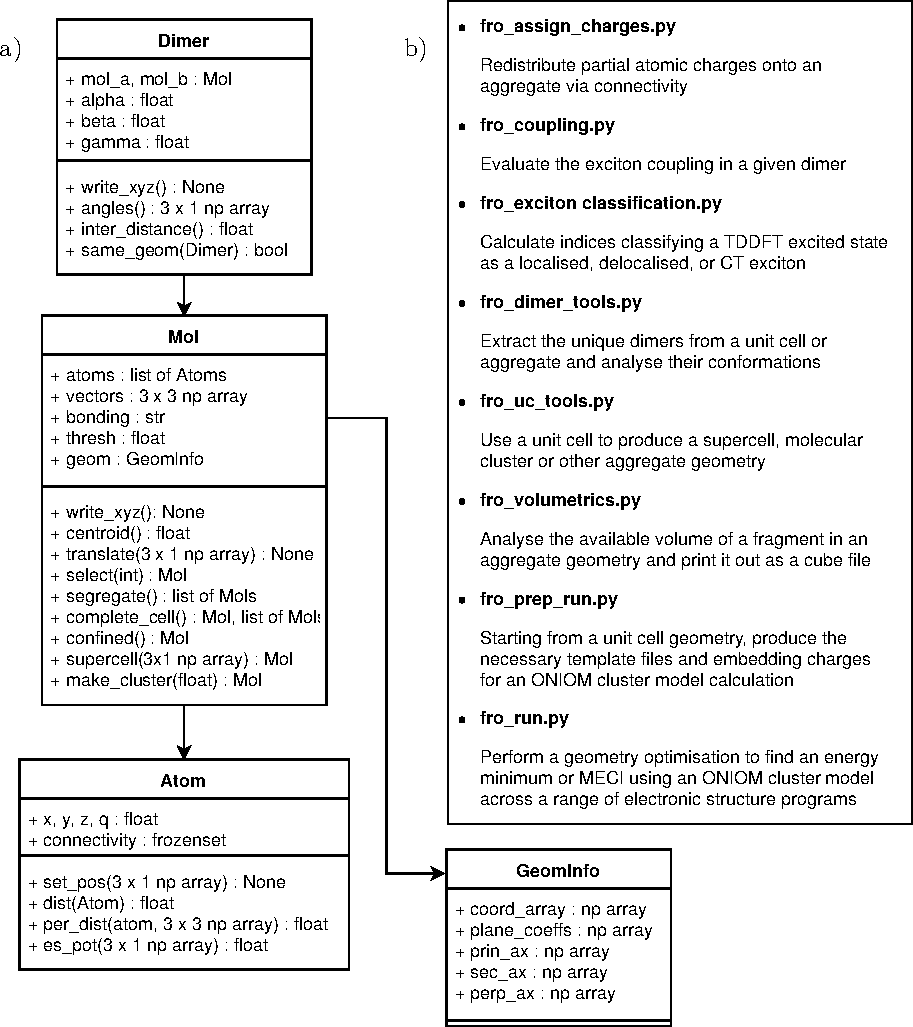
\includegraphics[width=12cm]{Chapters/6Implementation/classes.pdf}
  \caption{a) Principal class diagram of \texttt{fromage} b) Description of the main callable modules.}
  \label{fig:classes}
\end{figure}

\subsection{Dependencies}

The most common calculation performed by the geometry manipulation routines is the evaluation of interatomic distances. Therefore, for an overall speedup, these distances are calculated in C++ and wrapped as a Python function using SWIG. Some other more involved operations are sped up by using the \texttt{numpy}\cite{numpy} library. Geometry optimisation is carried out with the BFGS implementation in \texttt{scipy}.\cite{scipy}

The program \texttt{Ewald} by Derenzo \textit{et al.}\cite{Derenzo2000,Klintenberg2000} is used for the fitting of point charges to the Ewald potential. It is modified to allow the use of partial charges and redistribution with permission from the authors here https://github.com/Crespo-Otero-group/Ewald.

\section{Features}
\label{sec:features}
\subsection{Geometrical Analysis}
\subsubsection{Voronoi Volumes}
\label{sec:vor}

The conformational freedom of a molecule in the gas phase is only limited by its structural features and how they relate to the potential energy surfaces  (PES) of particular reaction coordinates. The electronic excitations within a molecule can in general be rationalised by scrutinising and comparing its different PESs. In contrast, in condensed phases, a molecule's freedom of nuclear reorganisation is hindered by the close packing imposed by its environment. The study of the effect of this close packing on excited state PESs and photochemical behaviour is a vast topic and involves an accumulation of inter-related factors both electronic and nuclear in nature which are often hidden behind the deceptively concise term of \textit{steric hindrance}.\cite{Dommett2017c,Blancafort2018}

It is however appropriate to begin such an investigation by obtaining computationally inexpensive and easily interpretable features of the packing of the aggregate. A routine approach for crystals is dividing the unit cell volume by the amount of molecules in the cell to find the average volume $V_{c}$ assigned to the molecule within the packing pattern in order estimate the tightness of packing. However this volume is difficult to compare between crystals composed of different molecules and is not visualisable. The determination of Voronoi volumes for molecules in aggregate is a promising alternative.

\begin{figure}[ht]
\centering
  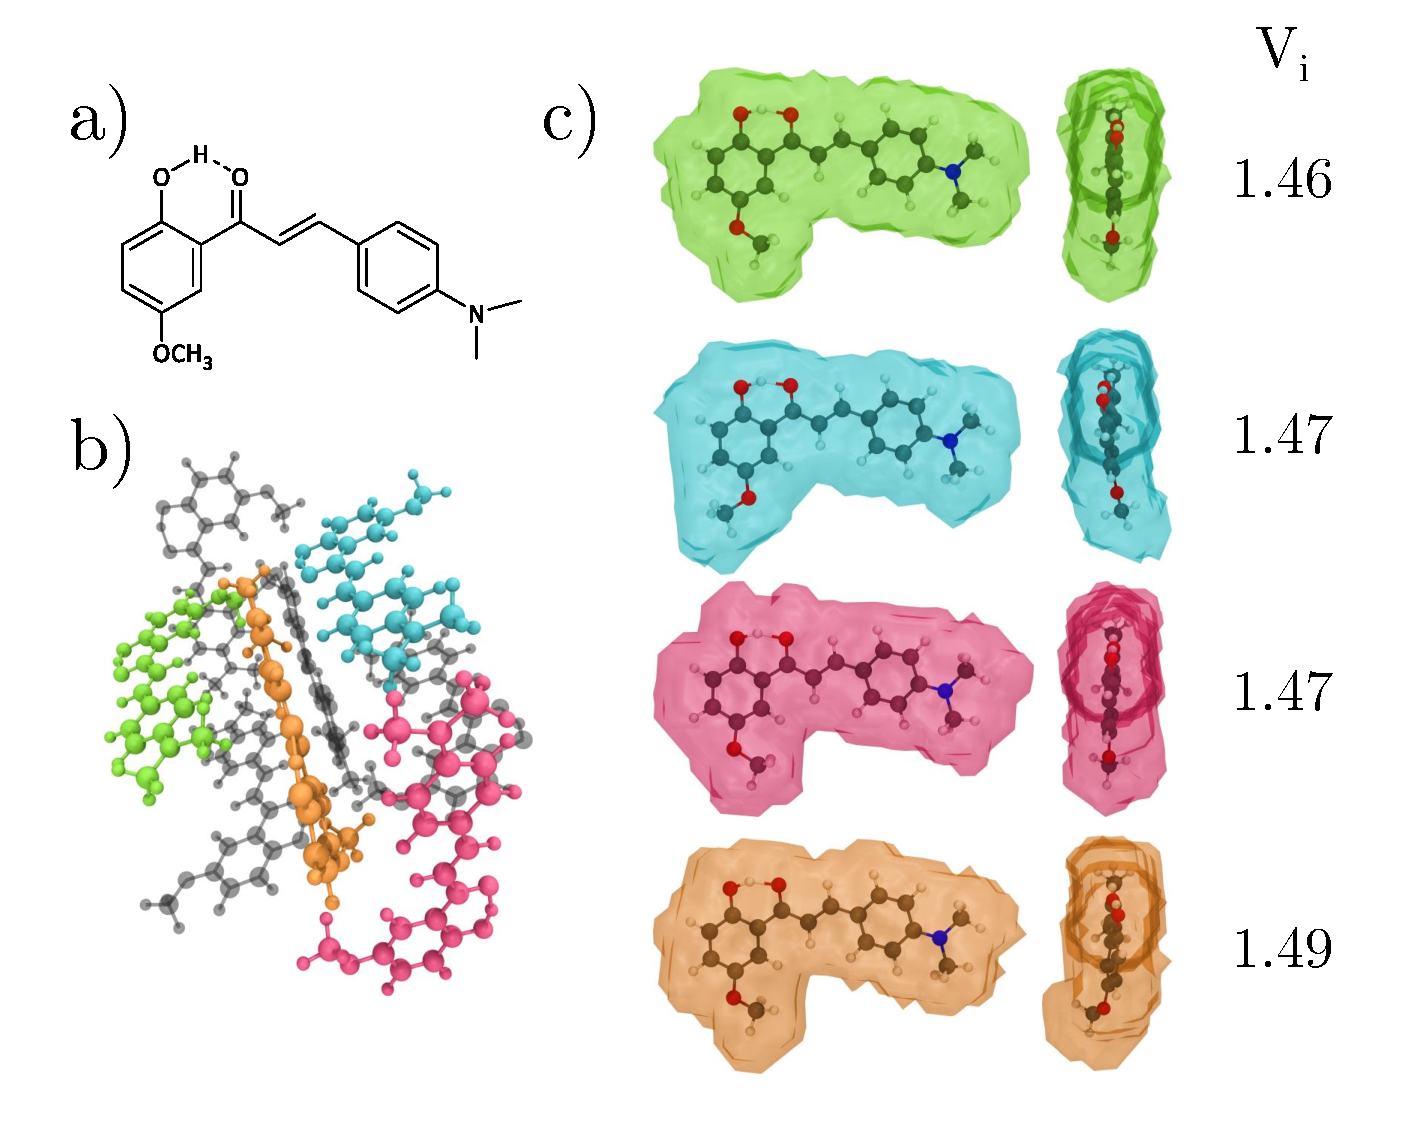
\includegraphics[width=10cm]{Chapters/6Implementation/vols.pdf}
  \caption{a) Chemical structure of HC2 b) unit cell of the HC2 crystal with the asymmetric cell highlighted by colour c) Profiles of the Voronoi volumes for the four molecules of the asymmetric cell with their volume index.}
  \label{fig:vols}
\end{figure}

In an aggregate of atoms a point belongs to the Voronoi volume of a given molecule if the atom it is nearest to belongs to that molecule. The application of Voroni cells\cite{Voronoi1907} to molecular systems has successfully been used to characterise the geometry of condensed phases\cite{Procacci1992} and notably liquids.\cite{Hunjan2010} This definition is refined by scaling the distance metric by the van der Waals radius of the atom; thus, for instance, assigning more space to oxygen than to hydrogen. For the calculation of distances, we employ a grid based scheme, which makes it robust and allows us to choose an arbitrary resolution for the volume.\cite{Abascal2013,Menzl2016} The resulting Voronoi volume $V_V$ can be compared to the sum of the van der Waals spheres of the atoms in the molecule (counting their intersection only once) $V_{vdW}$ to obtain a volumetric index $V_i = \frac{V_V}{V_{vdW}}$ which gives a normalised indication of the tightness of packing in the crystal for a specific molecule.

The Voronoi volumes introduce a distinction between inequivalent molecules in a crystal, and in fact should average out to $V_{c}$ if the $V_V$ values are weighted by the amount of occurrences of the molecule per unit cell. They can be used in finite systems such as amorphous clusters and perhaps most importantly, they are visualisable. Seeing the shape of a Voronoi volume can indicate the available space in the aggregate and therefore the areas of the PES least restricted by the environment.

A user may open a cluster geometry file \texttt{clust.xyz} with a visualising program and choosing which molecule they wish to calculate the Voronoi volume of with \texttt{fromage}. They identify the molecule by marking down the label of any atom belonging to the molecule. Then, upon calling:
\begin{verbatim}
fro_volumetrics.py clust.xyz -l [atom label]
\end{verbatim}
the program will generate the files \texttt{voro.cube}, \texttt{vdw.cube} and \texttt{union.cube} which are the visualisable Voronoi and van der Waals volumes of the molecule, and their union (in the set theory sense). A file called \texttt{volumes} contains the integrated volume of each of these.

An illustrative example is a derivative of 2'-hydroxychalcone (HC1), which upon the addition of a methoxy group in \textit{para} position with respect to the hydroxyl group turns off its emissive character in crystal form, bringing the fluorescence quantum yield from 0.32 to less than 0.01.\cite{Zhang2015,Zahid2017} The new molecule is HC2, discussed in Chapter \ref{chap:jctc}. While HC1 exhibits herringbone style packing, HC2 has a complex unit cell structure whose steric constraints on the individual molecules are unclear at first glance. Figure \ref{fig:vols} shows the difference in tightness of crystal packing between inequivalent monomers of HC2.

\subsubsection{Dimeric Arrangement}
\label{sec:dimer_axes}
Excitations in molecular aggregates are not guaranteed to remain confined to one absorbing monomer. Indeed, the electronic wavefunctions of the neighbouring molecules may have enough intermolecular overlap to produce intermolecular electronic interferences in the excited state. This can manifest in all sorts of photochemical processes and is central to exciton governed mechanisms like charge transfer or singlet fission. In crystals, typical packing motifs like herringbone or sheet-like, produce a limited set of archetypal dimer arrangements such as edge-to-face or face-to-face which have generalisable excitonic behaviour for chemically similar molecules.\cite{Kasha1965,Dommett2019} For instance in face-to-face aromatic systems, $\pi\pi$ interactions are a defining feature of the excitonic states.

Regardless of whether a researcher is investigating an amorphous cluster or a crystal structure, it is therefore informative to extract all of the significant dimers in the system and to quantify their geometrical arrangement in order to classify them under the principal dimer archetypes at a glance. In \texttt{fromage}, the user can extract the possible dimers whose distance falls below a given threshold. The intermolecular distance can be defined either as the centroid-to-centroid distance or as the nearest intermolecular atom pair distance. The latter can also be complemented by the van der Waals radii of the atoms. If the molecules are in lattice positions, the symmetry of the unit cell will produce groups of dimers identical up to a reflection or rotation. To filter out repeated configurations, all the intermolecular atomic distances are evaluated and sorted which provides a fingerprint for the dimer geometry. Equivalent dimers are then defined as ones with the same fingerprint up to an RMSD threshold of $10^{-4}$ \AA{} by default.

The dimeric arrangement can then be characterised quantitatively. An orthonormal set of principal, secondary, and tertiary axes is calculated for each constituent fragment and the angles between same axes of two molecules can be associated to an archetypical dimer, effectively classifying the pair.


The generalised procedure to obtain characteristic vectors for a molecule is shown in Figure \ref{fig:vectors}:
\begin{enumerate}
    \item All atoms of the molecule are projected onto an averaged plane by singular value decomposition.
    \item The two longest interatomic distances are identified, forming a quadrilateral $ABCD$ such that $AC > BD$ and $AB$ is the longest side. This imposes an arbitrary but consistent direction for the vectors.
    \item The following midpoints are detected: [AB]$\rightarrow${}H; [BC]$\rightarrow${}G; [CD]$\rightarrow${}F; [DA]$\rightarrow${}E. The principal and secondary vectors $\vec{a}$ and $\vec{b}$ respectively go from E to G and F to H.
    \item The two vectors are normalised and rotated equally until they are perpendicular. The tertiary vector is $\vec{c} = \vec{a}\times\vec{b}$.
\end{enumerate}

\begin{figure}[ht]
\centering
  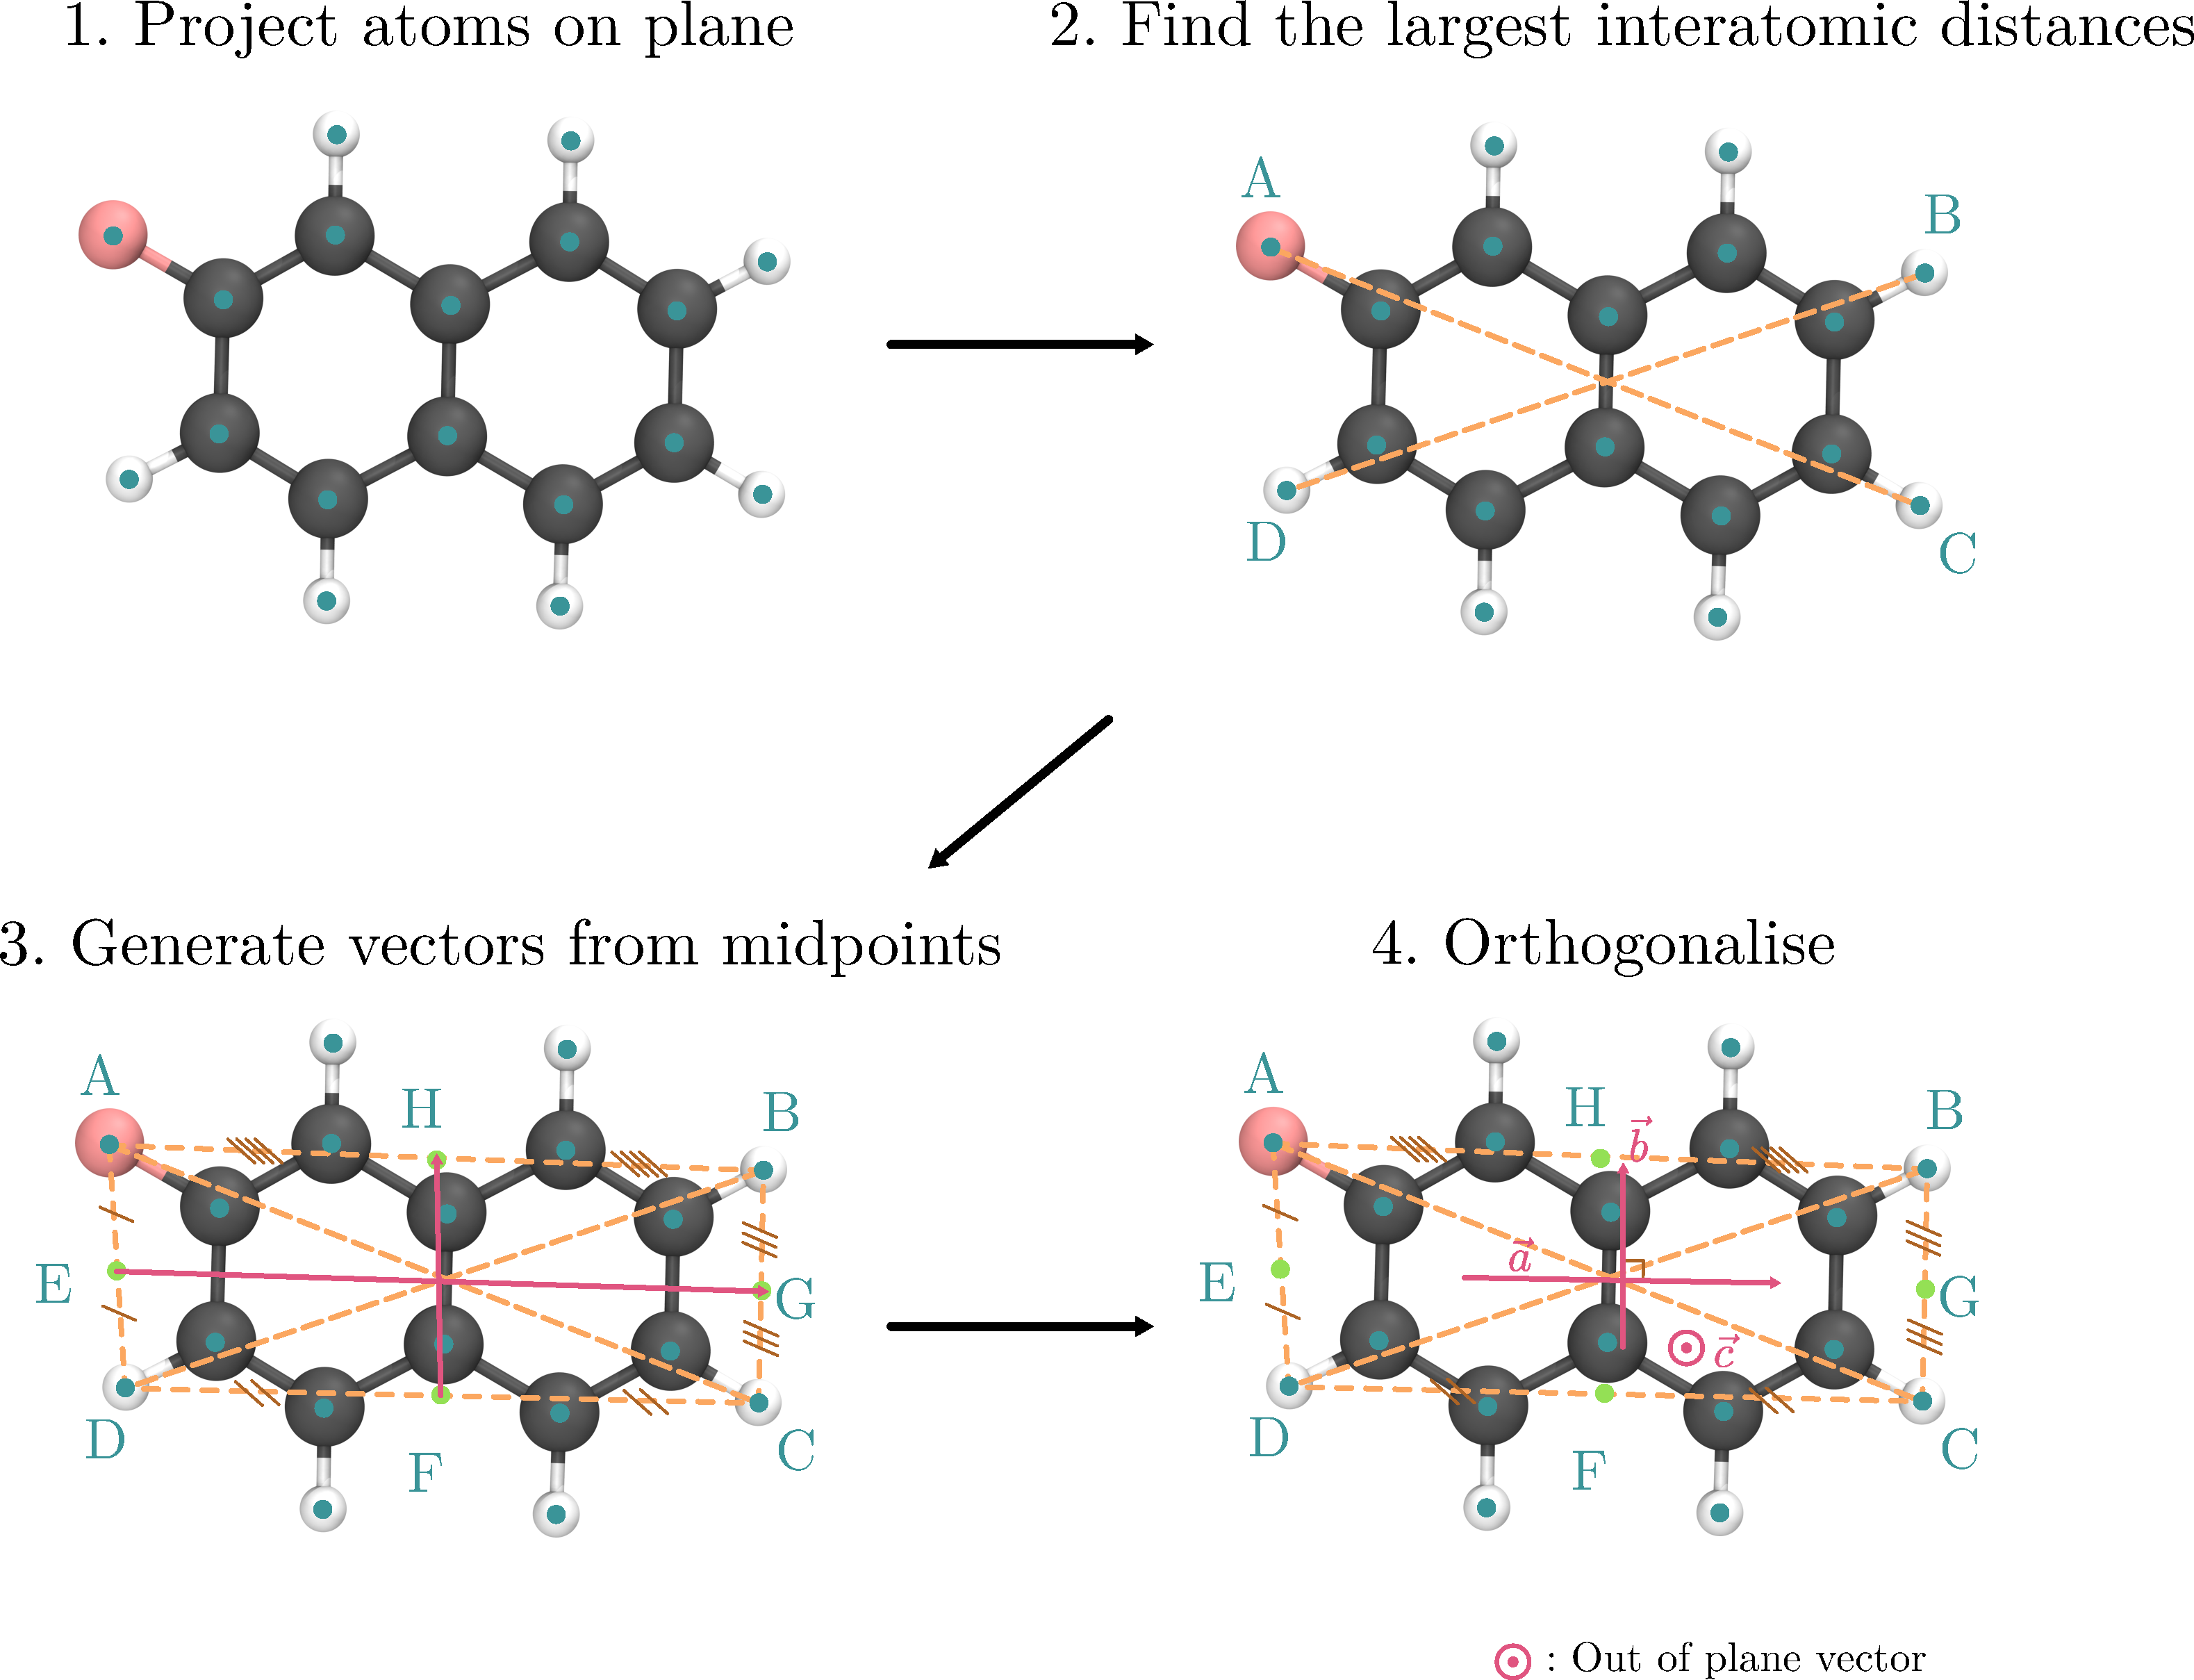
\includegraphics[width=9cm]{Chapters/6Implementation/vectors.pdf}
  \caption{Algorithm to generate principal axes from a monomer geometry with 2-fluoronaphthalene as an example.}
  \label{fig:vectors}
\end{figure}

This orthonormal set of axes presumes the significance of a plane which defines the shape of the molecule. Conjugated organic systems, those with optical applications, are often planar due to their aromatic components.\cite{Gierschner2016} In other cases, the judicious elimination of extraneous atoms from the analysis\textemdash{}a feature present in the code\textemdash{}can reduce the significant coordinates to a plane. To exclude a particular atom type from the calculation, only one atom need be specified, and others with the same identity can be automatically detected using the method outlined in section \ref{sec:prog_oniom}. 

If one same atom is involved in both largest interatomic distances, the procedure remains valid and the points C and D become degenerate. In certain cases, the principal axis should simply be the vector connecting the largest interatomic distance. When this option is selected, the secondary axis becomes the perpendicular axis which lies on the averaged plane. In the general case where one wishes to extract the geometric information from a cluster of dimers \texttt{clust.xyz}, one should use the command:
\begin{verbatim}
    fro_dimer_tools.py clust.xyz
\end{verbatim}
which will return the file \texttt{dimers.dat} containing all of the angles between dimers, the centroid distances and a proposed classification into different archetypical dimers. An additional slip angle is printed, to estimate the amount of face-to-face overlapping area giving rise to $\pi\pi$ interactions. It is defined as the smallest angle between the centroid-to-centroid axis and either tertiary axis of the constituent monomers, as is discussed in Ref. \citenum{Dommett2019}.

\begin{figure}[ht]
\centering
  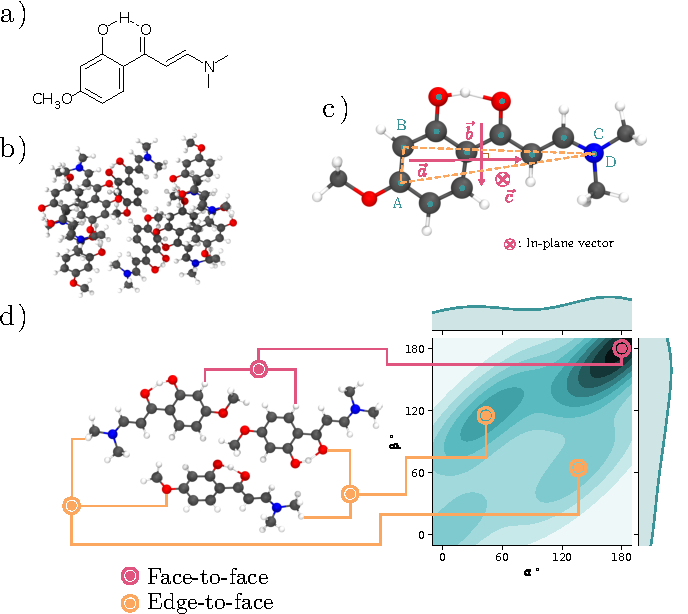
\includegraphics[width=9cm]{Chapters/6Implementation/hp3.pdf}
  \caption{Case study of DMAH for dimer geometry analysis a) Chemical structure b) Crystalline cluster c) Principal axes determination d) Heatmap of the angles between primary and secondary axes, respectively $\alpha$ and $\beta$.}
  \label{fig:angles_setup}
\end{figure}

\sloppy{
 The above method was used to investigate (2E)-3-(dimethylamino)-1-(2-hydroxy-4-methoxyphenyl)-2-propen-1-one (DMAH).} This molecule exhibits lasing behaviour with a fluorescence quantum yield of 0.77 in crystal form compared to 0.19 in PMMA film.\cite{Tang2016a} The crystal structure was optimised in \texttt{Quantum Espresso} using PBE-D2 with a plane-wave cutoff of 30 Ry and a 8x6x6 k-point mesh. A cluster of molecules was extracted from its crystal positions and all dimers with centroids falling less than 10 \AA{} from each other were considered. In this case, certain nonessential atoms were ignored in the geometric analysis and the points B and C became degenerate. The results are represented on Figure \ref{fig:angles_setup}. The points at (44\degree{},115\degree{}) and (136\degree{},65\degree{}) have a large $\beta$ which is characteristic of the edge-to-face dimers in herringbone packing. However the $\alpha$ values are unusually far from 0\degree{} or 180\degree, showing a packing arrangement specific to this crystal. The point at (0\degree{},0\degree{}), is in this case only related to the dimers which monomers form with periodic images of themselves.


\subsection{Exciton Analysis}


\subsubsection{Exciton Classification}

The exciton model is a framework to characterise different types of many-body electronic excitations in collections of molecules. The excitation can be associated with a localised Frenkel exciton, or a charge-transfer state, which are characterised by the electron density respectively migrating intra- and intermolecularly. A delocalised Frenkel excitation corresponds to an electron density reorganisation throughout the dimer with no net charge transfer. Differentiating between these three behaviours is crucial for the design of organic semiconductors in solar cells, since the process of charge separation and migration is fundamental to their mechanism. One approach is that of analysing the one-electron transition density matrices associated with the excitation, which contains information about the migration of the charge during the process.\cite{Plasser2012} This method is implemented in \texttt{TheoDORE}.\cite{plasser2017theodore}

Refs. \citenum{Crespo-Otero2012} and \citenum{Sen2013} propose a different scheme to qualify the nature of the exciton by comparing the charge density distribution on fragments of a dimer before and after excitation. The original implementation is in a program named \texttt{CALCDEN} which combines Perl and Fortran. The reimplementation in \texttt{fromage} is Python importable, making it an attractive alternative for use and extension depending on the user's preference.

A Mulliken partition scheme can supply integrated orbital-specific density coefficients located on one molecule ($A$):
\begin{equation}
    \rho^k_A = \sum_{\mu \in A, \nu \in A} c_{\mu k} c_{\nu k} S_{\mu \nu} + \sum_{\mu \in A, \nu \in B} c_{\mu k} c_{\nu k} S_{\mu \nu}
\end{equation}

$S_{\mu \nu}$ is the overlap integral between basis functions $\phi_{\mu}$ and $\phi_{\nu}$, and $c_{\mu k}$ is the coefficient of basis function $\phi_{\mu}$ in molecular orbital $k$. This density coefficient, $\rho^k_A$, can be used to produce two indices related to an excitation $I$:

\begin{equation}
\begin{split}
    \Sigma P^I_A = \sum_{i\rightarrow{}j} \sigma_{ij} (C^I_{i\rightarrow{}j})^2(\rho^j_A + \rho^i_A)\\
    \Delta P^I_A = \sum_{i\rightarrow{}j} \sigma_{ij} (C^I_{i\rightarrow{}j})^2(\rho^j_A - \rho^i_A)
\end{split}
\label{eq:exciton}
\end{equation}

Where $C^I_{i\rightarrow{}j}$ is the TDDFT coefficient corresponding to the excitation from orbital $i$ to $j$ and $\sigma_{ij}$ is $1$ for $i<j$ and $-1$ for $i>j$, in the case of de-excitation. These indices are in units of $\mathrm{e^-}$ and since they are associated to one excited state only, they have bounds $0 \leq \Sigma P^I_A \leq 2$ and $-1 \leq \Delta P^I_A \leq 1$. $\Sigma P^I_A$ represents the amount of electrons changing populations of atomic orbitals within $A$ for a given excitation. $\Delta P^I_A$, on the other hand, represents the electrons from $A$ populating atomic orbitals of $B$ ipon excitation, or \textit{vice versa}.

The combination of the two quantities indicates the behaviour of the electronic density upon excitation; a large reorganisation of density confined to molecule $A$ (labelled \texttt{LOC(A)}) would manifest in an extreme $\Sigma P^I_A$, closer to 0 $\mathrm{e^-}$  for molecule $B$ and closer to 2 $\mathrm{e^-}$  for molecule $A$. On the other hand, extreme $\Delta P^I_A$ values indicate a net loss or gain of density by one molecule. Values closer to -1 $\mathrm{e^-}$ correspond to a charge transfer from A to B (\texttt{CT(A→B)}) and \textit{vice versa} for values close to 1 $\mathrm{e^-}$. If none of the indices have extreme values, the excitation is delocalised, labelled \texttt{DELOC}. In \texttt{fromage}, an arbitrary threshold is in place by default where an excitation less than 0.5 $\mathrm{e^-}$ from an extreme value is classified as the corresponding type of exciton.

This method inherits the limitations of Mulliken population analysis, and basis set superposition, but has the advantage of only relying on TDDFT coefficients and overlap matrices, making it much faster than methods which investigate the spatial features of the density difference between excited and ground state.

\begin{figure}[ht]
\centering
  \includegraphics[width=7cm]{Chapters/6Implementation/classification.pdf}
  \caption{Transition density of two excited states of a perylene dimer taken from its crystal structure. The excited state energies are reported with respected to S$_0$. The electron density migrates from the blue to the yellow areas upon excitation. The exciton classification indices are defined in equation \ref{eq:exciton} and are in units of $\mathrm{e^-}$.}
  \label{fig:classification}
\end{figure}

To evaluate the two indices and classify an excitation, the user should first perform a TDDFT or CIS calculation of the dimer. Currently, only \texttt{Gaussian} calculations are supported. They should ensure that the atoms of molecule A appear before those of B in the geometry field and that an \texttt{rwf} file is produced by using the option \texttt{\%rwf=[name].rwf}. Then, given the output files \texttt{tddft.log} and \texttt{tddft.rwf}, the command line:
\begin{verbatim}
fro_exciton_classification.py tddft.log tddft.rwf [number of excitation]
\end{verbatim}
will print out the values of $\Sigma P^I_A$ and $\Delta P^I_A$ along with a suggested classification (\texttt{DELOC}, \texttt{LOC(A)}, \texttt{LOC(B)}, \texttt{CT(B→A)} and \texttt{CT(A→B)}).

To illustrate the use of this feature, a dimer of perylene was extracted from its experimental crystal structure.\cite{Botoshansky2003} Its excited states were calculated in \texttt{Gaussian16} using TD-$\omega$B97X-D\slash{}6-31G(d), and the transition densities analysed using the orbital specific Mulliken partition scheme. The states S$_3$ and S$_4$ each had extreme values of the classification indices, with $\Sigma P^3_A = 0.95$ $\mathrm{e^-}$ and $\Delta P^3_A = 0.90$ $\mathrm{e^-}$ for the former, indicating a charge transfer from fragment B to a, and $\Sigma P^4_A = 1.88$ $\mathrm{e^-}$ and $\Delta P^4_A = 0.07$ $\mathrm{e^-}$ for the latter, corresponding to a transition confined to monomer A. Figure \ref{fig:classification} corroborates this classification by showing the electronic transition density of a \texttt{DELOC} S$_1$ and comparing it to the \texttt{CT(B→A)} S$_3$ and \texttt{LOC(A)} S$_4$.




\subsubsection{Exciton Coupling Evaluation}
\label{sec:detail_js}
The coupling associated with an exciton is a measure of the correlation between the individual isolated excitations within the exciton. Evaluating it can give us a quantitative bearing on the importance of the many-body effects in the excited state process.

Kasha's exciton model is the initial approach, reducing the electronic densities of the fragments to point dipoles and comparing their relative geometry.\cite{Kasha1965} Under the point dipole approximation (PDA), the exciton coupling between fragments $i$ and $j$ is expressed as:
\begin{equation}
J_{ij}^{\text{Kasha}} = \frac{\bm{\mu_i} \bm{\mu_j}}{R^3} - \frac{3(\bm{\mu_i}\cdot{}\bm{R_{ij}})(\bm{R_{ij}} \cdot{} \bm{\mu_j}) }{R^5}
\label{eq:pda}
\end{equation}
Where $\bm{\mu_n}$ is the electronic transition dipole moment for monomer $n$ and $\bm{R_{ij}}$ is the vector connecting the centroids of monomers $i$ and $j$.

For a better spatial resolution of the electrostatic interactions, one can instead calculate the interaction between atomic transition charges (ATC)\cite{Spano2016}:
\begin{equation}
J_{ij}^{\text{ATC}} = \sum_a^{N_i}\sum_b^{M_j} \frac{q_a q_b}{|\bm{R_a^i} - \bm{R_b^j}|}
\label{eq:atc}
\end{equation}
Where $\bm{R_c^k}$ is the position of atom $c$ of monomer $k$ with ATC $q_c$ and $N_k$ is the number of atoms of monomer $k$.

For more resolution, the transition electronic density itself can be used, yielding costly but exact Coulombic exciton coupling. Additional correction can be included, for example by including the dielectric response of the environment as a polarisable continuum model as is done in \texttt{EXAT}.\cite{Jurinovich2018}

These models are purely Coulombic in nature and do not take into account the short-range interaction affecting the excited state behaviour of adjacent molecules, which for example is dominant in charge-transfer states.

Aragó and Troisi have devised a procedure which evaluates the coupling $J_{ij}$ in a dimer by diabatising the Hamiltonian:\cite{Arag2015}
\begin{enumerate}
    \item Select an excited state property. For the sake of argument we will use the transition dipole moment (TDM) $\bm{\mu}$ but anything bearing relation to the excited electronic density would be applicable.
    \item Evaluate the property for the two lowest excited states, along with the energies, for the dimer. These are the adiabatic energies ($E^A_1$ and $E^A_2$) and adiabatic TDMs ($\bm{\mu}^A_1$ and $\bm{\mu}^A_2$).
    \item Evaluate the property for both isolated constituent monomers in the first excited state, retaining their orientation. These TDMs are labelled $\bm{\mu}^{ISO}_1$ and $\bm{\mu}^{ISO}_2$.
    \item Calculate the singular value decomposition $(\bm{\mu}^A)^*\bm{\mu}^{ISO} = \bm{U}\bm{\Sigma}\bm{V}^*$.
    \item Compute the matrix $\bm{C} = (\bm{UV}^*)^*$ which is the best unitary transformation matrix mapping the adiabatic to the diabatic basis.
    \item Compute the diabatic Hamiltonian:
\begin{equation}
\small
\label{eq:2j}
\begin{pmatrix}
E_{i}^D & J_{ij}\\
J_{ji} & E_{j}^D
\end{pmatrix}
=
\begin{pmatrix}
C_{11} & C_{12}\\
C_{21} & C_{22}
\end{pmatrix}
\begin{pmatrix}
E_{i}^A & 0\\
0 & E_{j}^A
\end{pmatrix}
\begin{pmatrix}
C_{11} & C_{12}\\
C_{21} & C_{22}
\end{pmatrix}
\nonumber
\end{equation}     

\end{enumerate}

The off-diagonal elements of the Hamiltonian the exciton coupling values $J_{ij}$. More details can be found in reference \citenum{Arag2015}. The diabatisation method has already been employed in \texttt{fromage} to investigate the aggregate behaviour of propeller-shaped emitters.\cite{Stojanovic2019}

We have further extended it to calculate $N$-dimensional diabatic Hamiltonians, thus, for example, allowing for the calculation of pairwise exciton coupling within a trimer in the excited state, taking into account the influence of the third monomer.

An additional approximate method is that of exploiting the exciton energy splitting of the molecular excited state upon formation of a dimer. In the dimer, the S$_1$ and S$_2$ states are separated by twice the magnitude of the exciton coupling, provided that the individual constituent molecules are in perfect resonance.\cite{Hsu2009} Even in less symmetric cases, this approximation has been used with reasonable success.\cite{Gierschner2013,Shi2017,Dommett2019}

\texttt{fromage} implements this half-gap method, the PDA Kasha model, the ATC Coulombic interaction model and the diabatisation scheme using either ATCs or TDMs as excited state properties.

The script \texttt{fro\_coupling.py} manipulates \texttt{Gaussian} log files to compute exciton couplings. Several schemes are implemented. For instance, if a user requires the diabatisation method using the TDM excited state property to find the diabatic Hamiltonian containing the first three couplings of a trimer, the steps would be as follows. Carry out \texttt{Gaussian} calculations of the S$_1$ states of the three constituent monomers and the first three excited states of the trimer, yielding the files \texttt{mon\_1.log mon\_2.log mon\_3.log} and \texttt{trim.log}. Then, use the command line:
\begin{verbatim}
fro_coupling.py -m DIA -p TDM -mf mon_1.log mon_2.log mon_3.log -nf trim.log -ns 3
\end{verbatim}

This will print out the diabatic Hamiltonian where the three lower triangular off-diagonal elements correspond to the three exciton couplings of the trimer.

As an illustrative example, the crystal structure of 1,4-bis-(4-styryl-styryl)-benzene (4PV) was used to extract inequivalent dimers and evaluate their couplings. The structure of 4PV has been experimentally shown to contain six monomers, departing from the high symmetry of an ideal herringbone crystal due to variable slight rotation of the extreme phenyl rings.\cite{VanHutten1999} First, the unit cell was optimised using PBE-D2 with a basis set cut-off of 50 Ry and a Monkhorst-Pack grid of 1x2x1 k-points as implemented in \texttt{Quantum Espresso}.\cite{Giannozzi2009} Then, the inequivalent dimers were detected by \texttt{fromage} using a centroid-centroid distance threshold of 7 \AA. The TDMs of these dimers were calculated using TD-$\omega$B97X-D\slash{}6-31G(d) in \texttt{Gaussian16}\cite{g16} and processed in \texttt{fromage} in order to evaluate exciton couplings using dimer and trimer diabatic Hamiltonians. The results are shown in Figure \ref{fig:4pv}. In this system, edge-to-face dimer arrangements have larger exciton couplings (97, 103 and 105 meV) than face-to-face ones (79 and 91 meV). The largest difference is of 26 meV which represents 25\% of the greatest coupling (105 meV). It is expected that in cofacial dimers with couplings of such magnitude, the short-range interactions should account for most of the coupling, making the use of a coupling scheme which accounts for exchange imperative.\cite{Fornari2017}

Overall, the inclusion of the third molecule in the trimer diabatic Hamiltonian reduces the magnitude of the couplings by about 10 meV which is significant since it is in the order of the difference between certain edge-to-face and face-to-face values.

The irregularities in the herringbone packing produce two different face-to-face dimers with respective centroid-centroid distances of 6.05 \AA{} and 6.15 \AA{}. This relatively small increase in distance reduces the exciton coupling by 12 meV (14\% of the average value), indicating that the natural packing of 4PV produces in dimers in an excitonically sensitive geometry.

\begin{figure}[ht]
\centering
  \includegraphics[width=11cm]{Chapters/6Implementation/dimer_js.pdf}
  \caption{a) Chemical structure of 4PV b) Top view of a cluster of 4PV molecules taken from their crystal positions c) Side view of the cluster with inequivalent dimers labelled by their exciton coupling value in meV. The values in parentheses are calculated as a trimer.}
  \label{fig:4pv}
\end{figure}

% In a trimer chromophore, $\textbf{H}^D$ becomes a 3x3 matrix
% \begin{equation}
% \small
% \label{equation: 3x3 diabatic matrix}
% \begin{bmatrix}
% E_{i}^D & J_{ij} & J_{ik}\\
% J_{ji} & E_{j}^D & J_{jk} \\
% J_{ki} & J_{kj}& E_{k}^D
% \end{bmatrix}
% =
% \begin{bmatrix}
% C_{11} & C_{12} & C_{13}\\
% C_{21} & C_{22} & C_{23}\\
% C_{31} & C_{32} & C_{33}
% \end{bmatrix}
% \begin{bmatrix}
% E_{i}^A & 0 & 0\\
% 0 & E_{j}^A & 0\\
% 0 & 0 & E_{k}^A\\
% \end{bmatrix}
% \begin{bmatrix}
% C_{11} & C_{12} & C_{13}\\
% C_{21} & C_{22} & C_{23}\\
% C_{31} & C_{32} & C_{33}
% \end{bmatrix}
% \end{equation} 


\subsection{ONIOM Calculations}
\label{sec:prog_oniom}
Whether it be to calculate an absorption or emission energy, locate nonradiative pathways, or build a potential energy surface, calculating an excited state electronic structure is an often unavoidable step in the study of molecular aggregates. This often proves to be challenging due to the environmental effects in such media.

As discussed in Chapter \ref{chap:emb}, hybrid method schemes can offer environmental corrections, where an active site calculated with a high accuracy method is embedded in an explicit environment of lower accuracy. Inter-program hybrid method codes are not uncommon. \texttt{GARLEEK}\cite{Pedregal2018} communicates between \texttt{Gaussian} and \texttt{Tinker} for subtractive QM:MM calculations. \texttt{Chemshell}\cite{Metz2014,Lu2019} provides additive QM:MM formulations. The Atomic Simulation Environment (ASE)\cite{Larsen2017} offers both additive and subtractive QM:MM as a Python library. However to our knowledge no such code yet offers inter-program ONIOM QM:QM' calculations in the excited state. \texttt{fromage} uses its interfaces with \texttt{DFTB+}, \texttt{Gaussian}, \texttt{Molcas}, and \texttt{Turbomole} to calculate energies and geometry optimisations of different kinds with ONIOM QM:QM'. Namely mechanical embedding, regular electrostatic embedding, Ewald point charge embedding, and self-consistent versions of the last two.

The point charges can originate from Mulliken or RESP calculations. To fit point charges to the Ewald potential, we use the \texttt{Ewald} program.\cite{Klintenberg2000,Derenzo2000,Weber2010} It was modified to allow for the use of noninteger charges and redistributed at \href{https://github.com/Crespo-Otero-group/Ewald}{https://github.com/Crespo-Otero-group/Ewald} with permission from the original authors, fulfilling the requirements of the Computer Physics Communications license.

The various quantum methods available and tested in \texttt{fromage} are listed in Table \ref{tab:methods} along with their corresponding programs.
\begin{table}
\centering
\caption{Interfaced quantum methods and their availability in electronic structure programs}
\begin{tabular}{lcccc}
    \toprule
    Method & DFTB+ & Gaussian & Molcas & Turbomole \\\midrule
    Hartree-Fock & \xmark & \textcolor[HTML]{589A21}{\cmark} & \xmark & \textcolor[HTML]{589A21}{\cmark}\\
    DFTB & \textcolor[HTML]{589A21}{\cmark} & \xmark & \xmark & \xmark\\
    DFT & \xmark & \textcolor[HTML]{589A21}{\cmark} & \xmark & \textcolor[HTML]{589A21}{\cmark}\\
    TDDFT & \xmark & \textcolor[HTML]{589A21}{\cmark} & \xmark & \textcolor[HTML]{589A21}{\cmark}\\
    ADC(2) & \xmark & \xmark & \xmark & \textcolor[HTML]{589A21}{\cmark}\\
    CC2 & \xmark & \xmark & \xmark & \textcolor[HTML]{589A21}{\cmark}\\
    CASSCF & \xmark & \textcolor[HTML]{589A21}{\cmark} & \textcolor[HTML]{589A21}{\cmark} & \xmark\\
    CASPT2 & \xmark & \xmark & \textcolor[HTML]{589A21}{\cmark} & \xmark\\\bottomrule
    \label{tab:methods}
\end{tabular}
\end{table}


Setting up hybrid method calculations is typically a technically tedious task, but as many steps as possible are automated in \texttt{fromage} while retaining the full flexibility of the interfacing programs. The line:
\begin{verbatim}
fro_prep_run.py
\end{verbatim}
accompanied with a few input files such as the unit cell and a configuration file, will prepare the template files for the actual calculations to follow. This may include cluster geometry generation, Ewald fitting procedures and self-consistent population analyses.

Then, if the user is satisfied with their newly generated embedded cluster, the line:
\begin{verbatim}
fro_run.py
\end{verbatim}
can perform geometry optimisation or single point calculations.

OEC, OEEC and SC-OEEC calculations all require the distribution of point charges from single molecule population analyses to aggregate geometries or unit cell structures. This is a routine operation for preparing forcefield calculations, where sets of atomic types are associated to a potential or another with predetermined charge values.\cite{Wang2004,Wang2006} The atomic type is usually dependent on its neighbouring bonded atoms and the bond types. For QM:QM' calculations, it would be more attractive to use a broader definition of the atomic type which distinguishes between same function atoms at nonequivalent parts of the molecule.

To this end, \texttt{fromage} implements a connectivity detection tool which reads population analysis information from a single molecule or unit cell calculation and redistributes it onto any other finite or periodic ensemble of same molecules. The procedure builds a bond order matrix $\mathbf{B}$ where $B_{ij}$ is the shortest path connecting atoms $i$ to $j$ in number of bonds. The construction of the matrix is represented in Figure \ref{fig:connectivity} and is performed as follows:
\begin{enumerate}
  \item Detect the first connections by computing all of the interatomic distances complemented by atomic radii.
  \item Check every zero element and detect atom pairs $(a,b)$ which have a connected atom $c$ in common, i.e. $B_{ac} \neq 0 \land B_{bc} \neq 0$.
  \item Assign $B_{ab} = B_{ac} + B_{bc}$.
  \item Repeat from step 2 until convergence of the matrix.
\end{enumerate}

An atom's identity can be completely defined by additionally using the element of the atom corresponding to each row of $\textbf{B}$. A sufficient fingerprint for a given atom is the amount of atoms of a given element which are located a certain amount of bonds away, accompanied by the atom's own element. For example a methyl hydrogen of methanol is sufficiently defined by stating that it is a hydrogen atom with one carbon atom one bond away, one oxygen atom two bonds away, two hydrogen atoms two bonds away and one hydrogen atom three bonds away.


\begin{figure}[ht]
\centering
  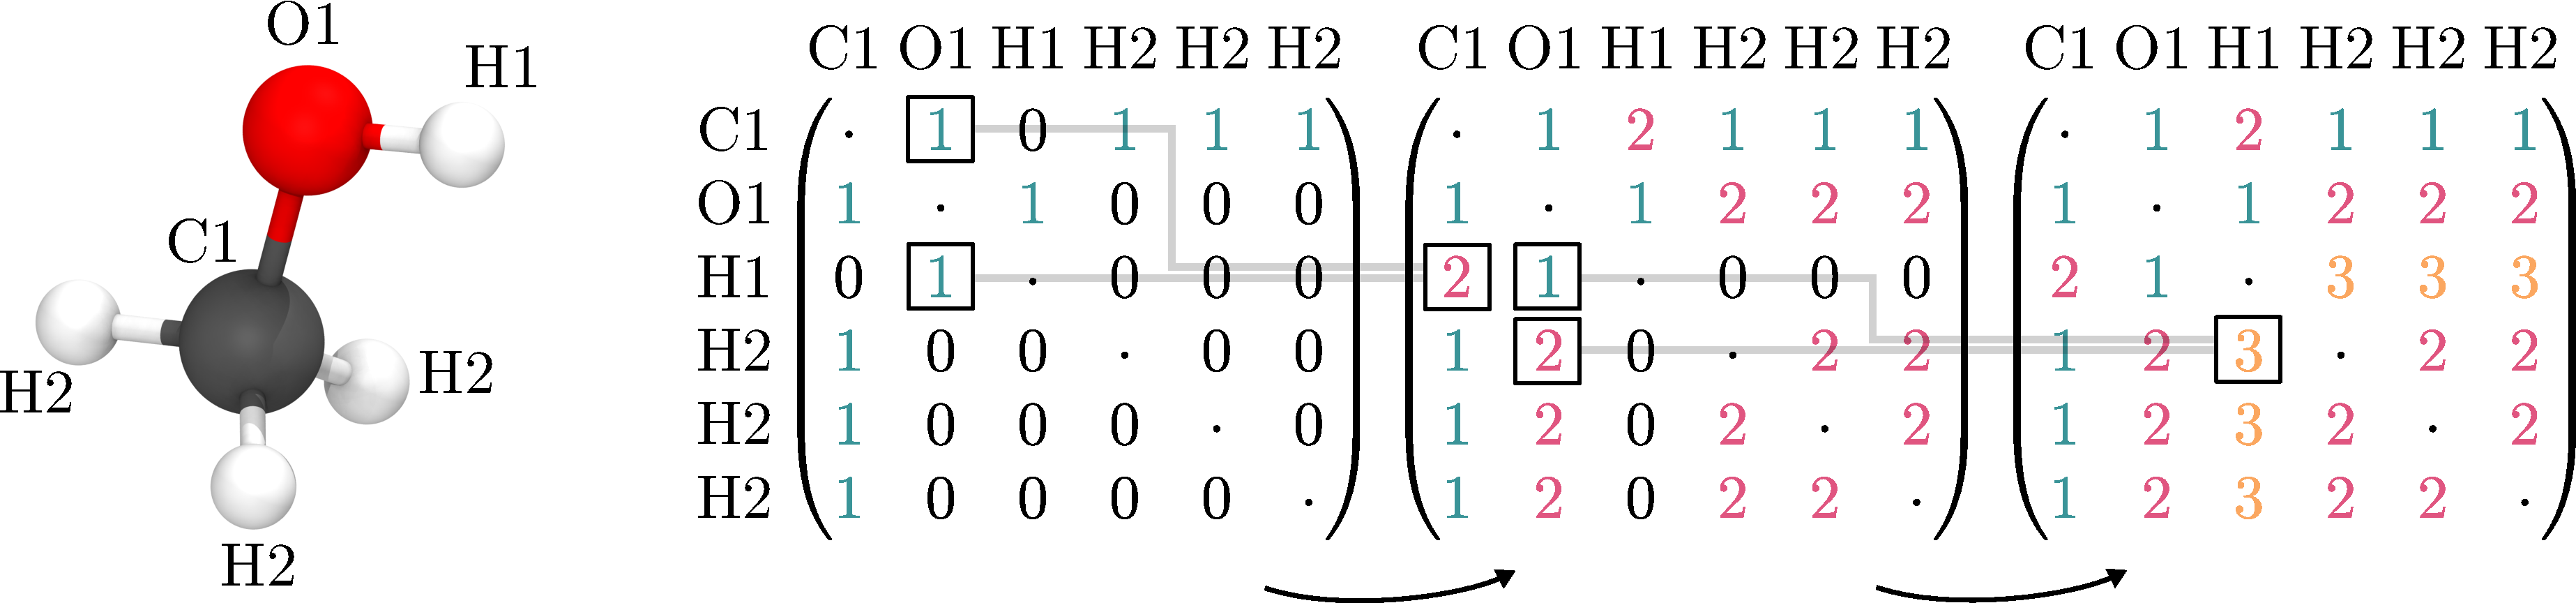
\includegraphics[width=\textwidth]{Chapters/6Implementation/matrices.pdf}
  \caption{Generation of the bond order matrix for methanol.}
  \label{fig:connectivity}
\end{figure}

Once all of the atomic identities are sampled from a reference molecule or unit cell, the partial charge values from this reference are distributed onto the desired target. When several reference atoms have the same identity (for instance three hydrogens belonging to the same methyl group), the average charge is retained. In practical terms, given for instance a Mulliken population analysis of methanol calculated in \texttt{Gaussian} with output file \texttt{pop.log}, and a Cartesian coordinate file of a cluster of methanol molecules \texttt{clust.xyz}, the line:

\begin{verbatim}
fro_assign_charges.py pop.log clust.xyz
\end{verbatim}
will produce a file \texttt{out\_char} which contains the coordinates of \texttt{clust.xyz} with an added column stating the partial charge of each atom.

All geometry optimisation routines use the the BFGS algorithm as implemented in \texttt{scipy}.\cite{scipy} To locate minima on the PES, the ONIOM energy expression (Equation \ref{eq:imomo}) is minimised. To locate conical intersections, the penalty function of Levine, Coe, and Mart\'inez is used instead (see Section \ref{sec:theo}).\cite{Levine2008}

\subsubsection{Example of Use}

The optimisation of excited state geometries in detailed condensed phase environments has numerous applications. For instance, the fluorescence of HC1 (see section \ref{sec:vor}) can also be switched off by the substitution of a methyl group in \textit{para} position with respect to the hydroxyl group, resulting in another dark compound: (2E)-3-[4-(Dimethylamino)phenyl]-1-(2-hydroxy-5-methylphenyl)-2-propen-1-one (DMAP).\cite{Zhang2015,Zahid2017}

Both HC1 and DMAP can experience excited state intramolecular proton transfer, splitting the excited state into two potential decay pathways. It was recently computationally shown that in HC, both the enol and the keto non-radiative decay pathways were rendered energetically inaccessible by a combination of molecular and crystalline factors.\cite{Dommett2017a,Dommett2017c}

OEEC was employed to investigate the critical points in the potential energy surface of DMAP. A thorough tutorial on how to perform these calculations is available here: \href{https://fromage.readthedocs.io/en/latest/tutorial.html}{https://fromage.readthedocs.io/en/latest/tutorial.html}. Geometry optimisations were carried out to locate the ground and excited state minima, as well as its Minimal Energy Conical Intersection Geometries (MECI). The crystal structure was optimised in \texttt{Quantum Espresso} using PBE-D2, a 40 Ry basis cutoff and a 1x2x1 k-point mesh. For the ONIOM calculation, the QM level of theory was TD-$\omega$B97X-D/6-311++G(d,p) while for the QM' level of theory, both HF/STO-3G and DFTB were employed. The energies and gradients were computed in \texttt{Gaussian16} for TDDFT and HF and in \texttt{DFTB+} for DFTB. Figure \ref{fig:pes_hc4} shows the relative energies of all the optimised critical points of the PES.

\begin{figure}[ht]
\centering
  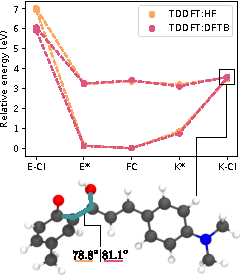
\includegraphics[width=6.5cm]{Chapters/6Implementation/hc4_fig.pdf}
  \caption{Relative energies of critical geometries of DMAP evaluated with OEEC at critical points of the PES. The Franck\textendash{}Condon point (FC), Enol (E*) and Keto (K*) excited state minima and Conical Intersection (CI) geometries were located.}
  \label{fig:pes_hc4}
\end{figure}

The enol non-radiative decay pathway is significantly above the absorption energy, rendering this channel inaccessible. On the other hand, the keto conical intersection is only about 0.2 eV above the absorption energy, arguably making it accessible \textit{via} thermal fluctuations. The availability of this nonradiative decay channel explains the low fluorescence quantum yield.

The TDDFT:HF and TDDFT:DFTB levels of theory have similar results, both in geometry and energy, with a difference of less than 0.1 eV at each point except form the enol MECI. This outlier can be attributed to the extreme bond stretching occurring between carbons in the back bond in the enol MECI conformation which would render both the Hartree-Fock formalism and the parameterisation of the DFTB calculations inadequate in differing ways. The striking agreement between the two methods is encouraging, given the relatively low computational cost of the semiempirical computation and the prevalence of HF as a ground state theory in QM:QM' protocols.\cite{Presti2014,Presti2016,Presti2016a,Presti2017}





\section{Conclusion}
We have detailed the principal capabilities of the Python library \texttt{fromage}, which aims to facilitate the computational investigation of the excited states of molecular aggregates. They include geometrical and exciton analysis as well as QM:QM' geometry optimisation tools, which have already been successfully employed in three past publications.\cite{Rivera2019,Stojanovic2019,Dommett2019} The features were tested on a diverse array of molecules, in order to challenge their robustness. They are implemented with enough flexibility that Python literate researchers can employ \texttt{fromage} scripts as part of a larger workflow with little added effort. By virtue of being an open source, unit tested and documented piece of software, \texttt{fromage} represents an addition to the fast expanding pool of sustainable chemical software libraries. We hope that by enabling researchers to use the framework and manipulate the source code, the field of aggregate photochemistry will continue to mature towards modern reproducible workflows.